\section{Neural networks setup}

\subsection{Artificial Neural Networks theory. \label{nn}}

The prior methods and materials described are essential to use Artificial Neural Networks (ANN) (Charu C. Aggarwal, 2018 \cite{livre_NN}, M. Albert, P. Besse, B. Laurent, 2020 \cite{cours_ML}). An Artificial Neural Network is non linear with respect to its parameters, noted as $\theta$, that associates to an entry $x$ an output $y = f (x, \theta)$. In this study, our output is uni-dimensional but it can be multidimensional in other applications.\newline

An artificial neuron, inspired by a biological neuron, is composed of : 
\begin{itemize}
    \item[\textbullet] a function $f_j$ of the input $x = \{x_1 \mbox{, ... , }x_d\}$
    \item[\textbullet] a vector of connection weights $w_j = \{w_{j,1} \mbox{, ... , } w_{j,d}\}$
    \item[\textbullet] a neuron bias noted $b_j$
    \item[\textbullet] an activation function $\phi_j$
\end{itemize}

This gives us : 
\begin{equation}
    y_j = f_j(x) = \phi ( <w_j , x> + b_j )
\end{equation}
Figure \ref{fig:neuron} represents an artificial neuron, where $\Sigma$ corresponds to $<w_j,x> + b_j$. 

\begin{figure}[H]
    \centering
    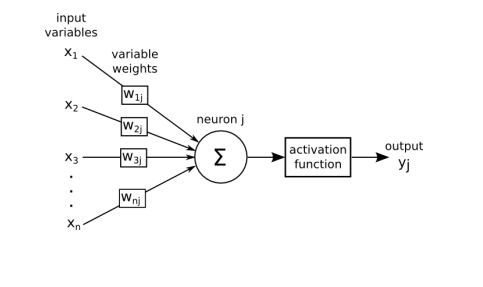
\includegraphics[scale = 1.1]{Graph/neuron.png}
    \caption{Schematic representation of an artificial neuron \cite{cours_ML}}
    \label{fig:neuron}
\end{figure}

A neural network, represented in Figure \ref{fig:neural_network}, is an association of several neurons, grouped in layers, called hidden layers. In this structure, also known as a multi-layer perceptron, the output of each neuron of a layer becomes the input of the neurons of the next layer. A potential different activation function than the hidden layers may be applied on the output layer depending on the problem, classification or regression. After having defined the architecture, we have to estimate the parameters, $w_j$ (grouped in matrix $W$) and $b_j$ (grouped in vector $b$), with a training sample and the back propagation algorithm. 

\begin{figure}[H]
    \centering
    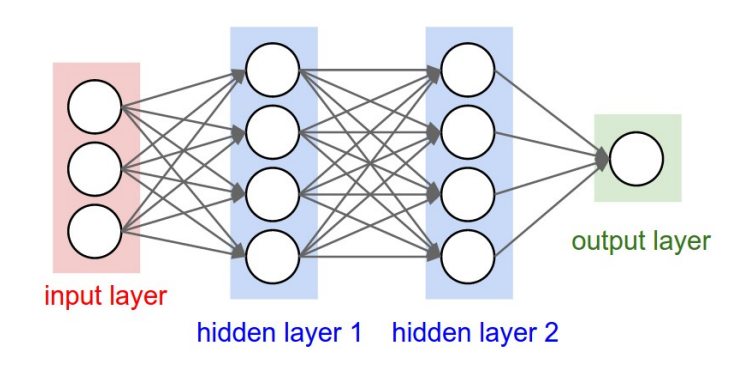
\includegraphics[scale = 0.7]{Graph/neural_net.png}
    \caption{Schematic representation of the architecture of a neural network \cite{cours_ML}}
    \label{fig:neural_network}
\end{figure}
A neural network is executed as follows : 
\begin{itemize}
    \item We select the explanatory variables used to train the network. The input data needs to be scaled whereas the output - the discharge in our case - does not need to be scaled. Then we split our dataset into a training set and a testing set, with a proportion of $80-20\%$.
    \item We choose a loss function. The main loss functions that we will use are Mean Absolute Error ($MAE$) and Mean Square Error ($MSE$). (See section \nameref{metrics})
    \item We randomly initialize the parameters $W$ and $b$. 
    \item We set $h^{(0)}(x) = x$. We compute at each hidden layer $k$, $h^{(k)}(x) = \phi (Wh^{(k-1)}(x)+b^{(k)})$ where $x$ is the input data. Then we compute the predicted values. This is the \textit{forward} phase. 
    \item We minimize a loss function, generally with a gradient descent algorithm, to find optimal $W$ and $b$. The gradient is computed with the backpropagation algorithm and the backpropagation equations. This is computed on subsets, called batches,  to optimize the computation time. Then, the values obtained are used to update the parameters $W$ and $b$. This is the \textit{backward} phase. 
    \item We iterate the \textit{forward} and the \textit{backward} phases a number of times called $epochs$ that we define.\newline
\end{itemize}

Le Cun (1986) \cite{lecun1989backpropagation} proposed the backpropagation algorithm which is an efficient way to compute the gradient of a neural network. It allows to easily obtain a local minimizer of the quadratic criterion. The idea is to recursively compute the gradient through the hidden layers. 

The success of the neural networks came from an universal approximation theorem due to Hornik (1991) \cite{hornik1991approximation}. This theorem shows that any bounded function can be approximated by a network with a single hidden layer, a finite number of neurons and a single activation function. 


\subsection{Long Short-Term Memory Networks.}

Long Short-Term Memory (LSTM) has been introduced by Sepp Hochreiter and Jürgen Schmidhuber in 1997 \cite{lstm_createur}. A LSTM is a Recurrent Neural Network (RNN). The main quality of a RNN and so of a LSTM network is that they can manage the time dependence contrary to classical neural networks.

To compute a RNN, we have to choose the number of memory layers, $K$. If $K$ is too big, the number of parameters increases too much. It becomes too complicated to learn the weights due to the vanishing gradient. RNN does not have a long term memory. In our case we need a long term memory. We must use LSTM networks.\newline

A LSTM includes an input gate, an output gate and a forget gate. A LSTM has its own memory $c$. Figure \ref{fig:lstm cell} shows the architecture at time $t$ of a LSTM cell.

\begin{figure}[H]
    \centering
    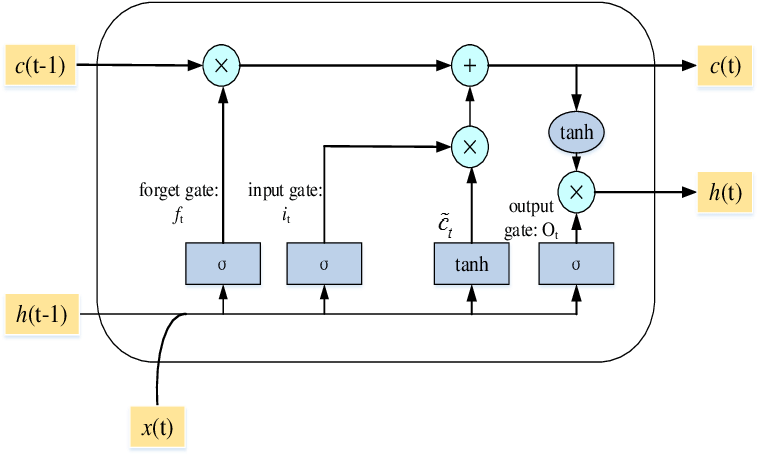
\includegraphics[scale = 0.4]{Graph/cellule_lstm.png}
    \caption{Schematic representation of a LSTM cell \cite{lstm_cell}}
    \label{fig:lstm cell}
\end{figure}

It works as follows :
\begin{itemize}
    \item The forget gate is used to "forget" useless information. $f_t = \sigma(W, [h(t-1), x(t)] + b_f)$
    \item The input gate proposes new information to put into the cell memory. $\tilde{C}_t = tanh(W, [h(t-1), x(t)] + b_f)$ corresponds to what information we put into the cell memory. $i_t = \sigma(W, [h(t-1), x(t)] + b_f)$ corresponds to the quantity of information we add.
    \item We use the two previous gates to compute the cell memory : $c(t) = c(t-1) f_t + i_t \tilde{C}_t $
    \item The output gate : $O(t) = \sigma(W, [h(t-1), x(t)] + b_f)$.
    \item Finally, $h(t) = O(t) + tanh(c(t))$ is calculated. It defines the output of the cell using the cell memory $c(t)$ and $tanh$ which determines what information to take from the memory.
\end{itemize}

Moreover, $\sigma$ is the sigmoid function, and $\{..., x_{t-1}, x_t, x_{t+1}, ... \}$ is the input time series.\newline

LSTM are linked in the way showed in figure \ref{fig:schema lstm}. In this illustration, we have 3 LSTM cells. 

\begin{figure}[H]
    \centering
    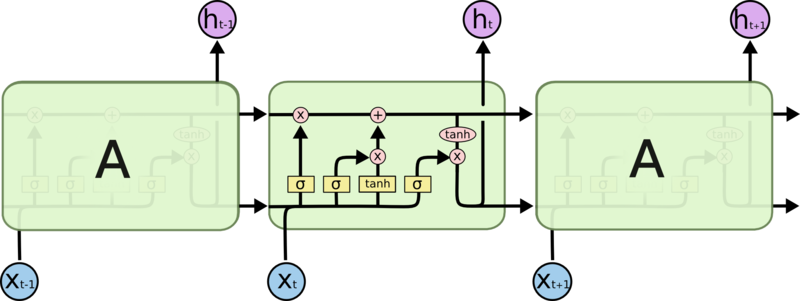
\includegraphics{Graph/schema_lstm.png}
    \caption{Schematic representation of the architecture of a LSTM network \cite{lstm-cell-linked}}
    \label{fig:schema lstm}
\end{figure}

To optimize the weight and the bias of each cell, we use the backpropagation of the gradient (detailed in previous section \nameref{nn}).

\subsection{Performance criteria. \label{metrics}} To evaluate the performances of a neural network, we quantify the errors using different criteria called metrics. 

\subsubsection{Useful common metrics.\label{section321}}
 We compute the \textit{Mean Square Error}, denoted by $MSE$, and defined in (\ref{eq:mse}).
\begin{equation}
    MSE(y) = {\frac{1}{n} \left( \sum^n_{i=1}(y^{est}_i - y^{obs}_i)^2 \right)}
    \label{eq:mse}
\end{equation}
with $y^{est}_i$ the $i^{th}$ estimation and $y^{obs}_i$ the true value associated.\\

\textit{Mean Absolute Error}, denoted by $MAE$ has a physical meaning, as it does not modify the values of the river discharge. Using the same notations as previous, $MAE$ is defined in (\ref{eq:mae}).
\begin{equation}
    MAE(y) = {\frac{1}{n} \left( \sum^n_{i=1}\lvert y^{est}_i - y^{obs}_i\rvert \right)}
    \label{eq:mae}
\end{equation}

 The \textit{Pearson correlation coefficient}, denoted by $R2$ is set in (\ref{eq:r2}).
\begin{equation}
    R2(y) = \frac{\sum_{i=1}^{n}(y^{est}_i - \bar y^{est}) (y^{obs}_i - \bar y^{obs})} {\left(\sum_{i=1}^{n}(y^{est}_i - \bar y^{est})^2\right)^{1/2}\left(\sum_{i=1}^{n}(y^{obs}_i - \bar y^{obs})^2\right)^{1/2}}
    \label{eq:r2}
\end{equation}

where $\bar y^{est}$ the average value of the estimations and $\bar y^{obs}$ the average value of the validation values.\newline

We define the \textit{Root Mean Square Error} in (\ref{eq:rmse}), denoted by $RMSE$ and the \textit{Normalized Root Mean Square Error}, denoted by $nRMSE$ in (\ref{eq:nrmse}).
\begin{equation}
    RMSE(y) = \sqrt {\frac{1}{n} \left( \sum^n_{i=1}(y^{est}_i - y^{obs}_i)^2 \right)}
    \label{eq:rmse}
\end{equation}

\begin{equation}
    nRMSE(y) = \frac{RMSE(y)} {\bar y^{obs}}
    \label{eq:nrmse}
\end{equation}

% \subsubsection{Useful metrics in hydrology.}

% Then, we define two other metrics specific to hydrology. The first one is the \textit{Nash-Sutcliffe model Efficiency}, denoted by $NSE$ and defined in (\ref{eq:nse}) with the same notations defined in \nameref{section321} section. The second one is the \textit{Kling-Gupta model Efficiency}, denoted by $KGE$ in (\ref{eq:kge}).
% \begin{equation}
%     NSE(y) = 1 - \frac{\sum^n_{i=1}(y^{est}_i - y^{obs}_i)^2} {\sum^n_{i=1}(y^{obs}_i - \bar y^{obs})^2}
%     \label{eq:nse}
% \end{equation}

% \begin{equation}
%     KGE(y) = 1 - \sqrt {(\beta_{KG}-1)^2+(\alpha_{KG}-1)^2+(R^2-1)^2}
%     \label{eq:kge}
% \end{equation}
% where $\beta_{KG}=\frac{\bar y^{est}}{\bar y^{obs}}$ and $\alpha_{KG} = \frac{\sigma(y^{est})}{\sigma(y^{obs})}$.

\subsubsection{Physical criteria : Low-Froude model.}

The last criteria we define is the Low-Froude model. The objective is to match physical criteria with a neural network. In our case, we want to know if the predicted river flow follows the Low-Froude model. The Strickler friction coefficient $K$ can be defined as a local power law (K. Larnier, J.Monnier, 2020 \cite{larnier2020hybrid}), i.e. for a given reach $r$ and an instant $p$, as shown in (\ref{eq:MS_law}): 

\begin{equation}
    K_{r,p} = \alpha_r \left( Z_{r,p} - Z{r,0} + \frac{1}{W-{r,0}}A_{0,r}\right)
    \label{eq:MS_law}
\end{equation}

where $\alpha$ and $\beta$ are Manning-Strickler coefficients.\newline

Using the Manning-Strickler law and (\ref{eq:MS_law}), (\ref{eq:low froude}) defines the algebraic Low-Froude flow model, a system of $R$ equations, where $R$ is the number of reaches : 
\begin{equation}
    Q^{3/5}_{r,p} = \alpha_r^{3/5} ( c_{r,p}^{(1)} A_{0,r} + c_{r,p}^{(2)})(c_{r,p}^{(4)}A_{0,r} + c_{r,p}^{(3)})^{3/5\beta_r}
    \label{eq:low froude}
\end{equation}
with : $ c_{r,p}^{(1)} = W_{r,p}^{-2/5}S_{r,p}^{3/10}$, $ c_{r,p}^{(2)} = c_{r,p}^{(1)} \partial A_{r,p}$, $ c_{r,p}^{(3)} = (H_{r,p} - H_{r,0})$, and  $ c_{r,p}^{(4)} = \frac{1}{W_{r,0}}$. These coefficients can be computed with altimetry measurements. 